\chapter{Modern Physics: Quantum Mechanics}

This first lecture opens in an unusual way. Instead of beginning with a formal postulate list, Leonard Susskind begins by explaining the style of the course and then turns at once to a deeper claim: quantum mechanics is not classical mechanics with a little noise stirred in. To make that point, he unfolds the subject in the order the lecture itself demands. We begin with classical randomness as a foil, then the two-slit experiment, then reversibility and the cost of looking, then Heisenberg's microscope, and only after that do we take the first abstract step toward complex vector spaces. Where board frames curated through LazyingArt LLC and Video2Book help stabilize equations or layout, they are retained as supporting evidence; the transcript remains the primary source for the sequence and force of the argument.

\section{Why This Course Starts With Logic, Not Machinery}

Susskind begins with the audience. This is not freshman service physics, and it is not a standard undergraduate or graduate course. It is a continuing-education course, and that fact shapes the method. The audience wants the basic ideas quickly, but not cheaply. We are to use equations when necessary, and when we do use them, we are to use the simplest equations that will actually do the job. He even jokes that one might call it quantum mechanics for old people, including himself. The joke matters less than the pedagogical point behind it: we are not here for ornament, but neither are we here for slogans.

That brief preface also explains why the lecture opens with logic rather than machinery. Susskind reminds us that classical mechanics came first in the larger sequence of courses, but quantum mechanics is more fundamental. Classical physics is what we get when quantum mechanics may be approximated by classical logic in the appropriate regime. So instead of starting with Schr\"odinger's equation or operator formalism, the lecture starts by asking what classical logic gets wrong. That is the right place to begin, because the mathematics introduced later is meant to replace a structure that has already failed.

\section{Classical Randomness Is Not Quantum Unpredictability}

The first task is to separate two ideas that are too easily conflated. Quantum mechanics certainly contains unpredictability. But that does not mean that it is simply classical mechanics plus random disturbances. To make the distinction sharp, Susskind invents a classical foil.

Imagine an otherwise Newtonian world in which a deity occasionally gives the moon tiny random kicks. Every tenth of a second the dice are thrown; on one outcome the moon is nudged one way, on another it is nudged the other way. This world would be statistically unpredictable, but the unpredictability would be of a familiar classical kind. It would enter by occasional deviations from deterministic law.

Now ask what such randomness would do. It would not merely blur our predictions. It would also jostle conserved quantities. If the kicks are random, then the energy of the system would, step by step, randomly increase or decrease. On average it might drift slowly or perhaps not at all, but exact conservation would be gone. The very form of the randomness would show itself in the energy bookkeeping.

Quantum mechanics does not behave that way. We prepare a system with a precise energy, let it evolve, and then measure again. The later result may be unpredictable in some respects, but the energy comes back exactly the same. No trace remains of a hidden hand knocking the system this way and that. So the lecture's first lesson is already in place: quantum unpredictability is highly special. It is not what one would get by sprinkling classical randomness into Newton's laws.

\section{The Two-Slit Experiment and the Failure of Additive Probabilities}

Susskind's first great example is the two-slit experiment, because it exhibits the weirdness of quantum mechanics in the most direct and least encumbered way. Let us follow the order of the lecture carefully.

We begin with a source of very light particles---photons, electrons, neutrons, anything for which quantum effects are appreciable. They are sent through the apparatus one at a time. This matters. The lecture insists on that sparsity precisely so that no later particle can plausibly be blamed for what happens to the earlier one.

First open only one small hole. A particle passes through and hits the screen in an isolated blip. Repeat the experiment many times and those individual blips build up a smooth profile: a bright central region fading away to the sides. We may call that one-hole distribution \(P_1(y)\). Close that hole, open the second one, and repeat. We obtain another profile \(P_2(y)\), displaced relative to the first.

At this stage classical logic seems irresistible. If both holes are open, then a particle reaching a point \(y\) on the screen must have come either through the first hole or through the second. Therefore the probabilities ought to add:
\begin{equation}
P_{12}(y)=P_1(y)+P_2(y).
\end{equation}
This is not the quantum rule. It is the classical expectation that Susskind wants fully on the table before overturning it.

Now do the real experiment. The particles still come one at a time. The screen still records one blip at a time. But the built-up pattern is no longer the sum of the two one-hole profiles. Instead we get an interference pattern, and at some points the probability vanishes entirely:
\begin{equation}
P_{12}(y)=0
\qquad \text{even though} \qquad
P_1(y)\neq 0,\quad P_2(y)\neq 0.
\end{equation}
This is the shock of destructive interference. With only the first hole open, particles arrive at that point. With only the second hole open, particles also arrive at that point. Open both holes, and no particle ever arrives there.

That is the point where Susskind widens the claim. One could try to invent some elaborate mechanism, some baroque memory hidden in the apparatus, but the phenomenon is too generic for that sort of one-off repair. The difficulty is not a local detail. The difficulty is that classical statistics and classical logic are built on the wrong underlying structure. The additive rule for alternatives has simply failed.

\section{Reversibility, Information, and the Cost of Looking}

Having displayed the failure of additive probabilities, the lecture shifts to a second diagnostic: reversibility. The move is deliberate. Susskind wants a different test, one that is not tied to slit interference, and for that he first backs up to very simple discrete systems.

Consider a two-state system, a coin with states \(H\) and \(T\). A deterministic law of motion can take the form
\begin{align}
H &\mapsto H, & T &\mapsto T,
\end{align}
or it can alternate the states,
\begin{align}
H &\mapsto T, & T &\mapsto H.
\end{align}
Now move to a three-state system with heads, tails, and feet:
\begin{equation}
H \mapsto T,\qquad T \mapsto F,\qquad F \mapsto H.
\end{equation}
The important point is not which law we choose. The important point is that in each of these examples the evolution is exact and information-preserving. If we let the system evolve for a long time and then reverse the arrows of the update rule, it retraces its history and returns to the starting state.

This gives Susskind an operational definition of reversibility. We do not need the detailed law; we need only the possibility of reversing it. Evolve for a time \(t\), reverse the rule, evolve for the same time \(t\) again. If the system always returns to its starting point, the dynamics is deterministic in the sense he wants.

Now add a tiny bit of classical randomness. Suppose that with some very small probability the system does not follow the prescribed update and instead does something else---for example, it stays put when the rule says move on. Over short times the reversal test may still succeed. But over sufficiently long times a fluctuation will almost certainly occur, and then running backward does not return us uniquely to the initial state. Information has been lost. That is why Susskind says that classical randomness destroys the conservation of information.

He now carries the same test over into quantum mechanics. Here the lecture momentarily wavers in its wording, but the logic is clear: for this thought experiment we no longer need two slits. One slit is enough. Send one electron through the slit. Remove the screen. Let the electron pass through, but do not detect it. Then reverse the law of physics and run the system backward for the same length of time.

What happens? If nothing has looked at the electron, nothing has recorded its location, nothing has disturbed it in the intermediate stage, then the reversal is exact. The electron retraces the reverse trajectory and goes back into the gun. That is already a remarkable statement. The apparent randomness of the one-slit deflection is not the same thing as classical random compounding of errors.

Now alter only one thing. Put in a detector and record where the electron is during the intermediate stage. Then reverse the law and run backward. In that case the exact return fails. The uncertainty does not cancel; it compounds. The reversibility test, which classical gentle measurement would have left untouched, is destroyed by quantum measurement itself.

This is the deeper transition of the lecture. Classical physics allows an arbitrarily gentle observation. One can, in principle, look at a classical system without significantly altering its subsequent behavior. Quantum mechanics does not. Determining the state of the system is never a harmless afterthought.

Susskind then returns to the two-slit experiment and states the same idea in a different form. The interference pattern is present only if nothing in the apparatus or environment records which slit the electron went through. That recorder need not be a human observer. It could be a gas molecule, another electron, or any degree of freedom that remembers afterward which path was taken. Once such path information exists in the environment, the interference pattern disappears and the answer reverts to the classical one: the probabilities add.

\subsection{Question \& Answer}

\paragraph{Question.} If the particle is deflected by the slit or plate, does the plate not recoil? And if it recoils, does that not already reveal which path the particle took?

\paragraph{Answer.} The recoil is real. The issue is whether it is readable. Susskind's answer is qualitative and deliberately anticipates the uncertainty principle before formally deriving it. A detector that is very well localized in position must have a broad momentum distribution. So although an electron gives the detector a small kick, that kick only shifts an already broad momentum distribution by a small amount. Unless the shift is comparable to the width of the distribution, one cannot tell afterward whether the kick occurred.

\begin{figure}[t]
\centering

\includegraphics[width=0.86\textwidth]{lecture_01_figure_02.png}
\caption{Board layout for the recoil argument. The broad central hump is the detector momentum distribution introduced in the answer; the large oval at left and the small triangle-like sketch at upper right are residual board context and should not be overread.}
\end{figure}

\begin{figure}[t]
\centering
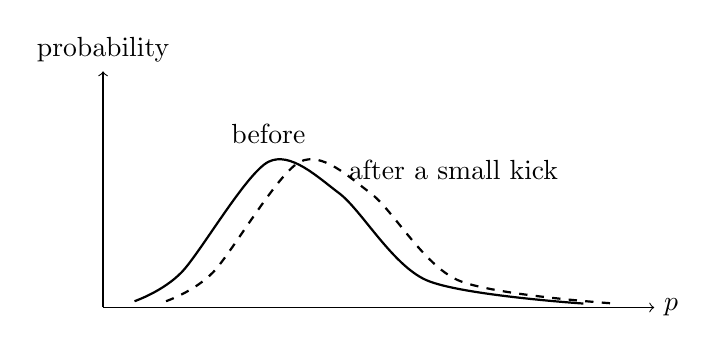
\begin{tikzpicture}[scale=1.0]
\draw[->] (0,0) -- (7.0,0) node[right] {$p$};
\draw[->] (0,0) -- (0,3.0) node[above] {probability};
\draw[thick] plot[smooth] coordinates {(0.4,0.08) (1.0,0.45) (2.1,1.85) (3.0,1.45) (4.1,0.35) (6.1,0.05)};
\draw[thick,dashed] plot[smooth] coordinates {(0.8,0.08) (1.4,0.45) (2.5,1.85) (3.4,1.45) (4.5,0.35) (6.5,0.05)};
\node at (2.1,2.2) {before};
\node at (4.45,1.75) {after a small kick};
\end{tikzpicture}
\caption{Transcript-derived redraw of the detector momentum distribution. The lecture's point is that a small recoil may shift the distribution without making that shift experimentally readable.}
\end{figure}

The lesson is precise enough for our purposes. Recoil does not automatically provide which-path information. It provides readable information only if the shift in detector momentum is large compared with the detector's own intrinsic momentum uncertainty.

\section{Heisenberg's Microscope and the Momentum of a Photon}

At this point Susskind turns explicitly to the uncertainty principle. But again he does not present it first as a formal theorem. He stages it as a demand for physical explanation. Heisenberg may say that position and momentum cannot be simultaneously determined, but Bohr's challenge is: do not merely tell me that \(x\) and \(p\) fail to commute; show me the physics that forces this obstruction.

The physical setting is measurement by light. To locate a particle under a microscope, we scatter a photon from it, collect the scattered light, and form an image. So the next question is simple: what did Einstein, de Broglie, Bohr, and Heisenberg know about photons that makes this measurement problematic?

The board snapshot is valuable here because it preserves the cluster of relations as Susskind arranged them.

\begin{figure}[t]
\centering

\includegraphics[width=0.86\textwidth]{lecture_01_figure_04.png}
\caption{Board layout for the photon-energy and wave-kinematics relations leading to the inverse momentum-wavelength law.}
\end{figure}

The first relation is Einstein's photon-energy formula:
\begin{equation}
E=hf=\hbar\omega,
\end{equation}
with
\begin{equation}
\omega = 2\pi f,
\qquad
\hbar = \frac{h}{2\pi}.
\end{equation}
Susskind then recalls that light carries momentum as well as energy. For ordinary nonrelativistic particles, one has
\begin{equation}
E=\frac{p^2}{2m}=\frac{1}{2}pv,
\end{equation}
so energy and momentum already have the right dimensions to be related by a speed. For light, the relativistic relation is simpler:
\begin{equation}
E=cp,
\qquad\text{hence}\qquad
p=\frac{E}{c}.
\end{equation}

Now combine this with the photon-energy formula:
\begin{equation}
p=\frac{hf}{c}.
\end{equation}
To eliminate the frequency we use the kinematics of a wave. If one cycle takes time \(T\), then
\begin{equation}
T=\frac{1}{f}.
\end{equation}
If the wavelength is \(\lambda\), then in one period the wave advances by one wavelength, so
\begin{equation}
c=\frac{\lambda}{T}=\lambda f,
\qquad\text{or equivalently}\qquad
f=\frac{c}{\lambda}.
\end{equation}
Substituting into the momentum relation gives the de Broglie formula:
\begin{align}
p &= \frac{hf}{c}
   = \frac{h}{c}\frac{c}{\lambda}
   = \frac{h}{\lambda}.
\end{align}
This is the decisive step: momentum and wavelength are inverse to one another.

The lecture then pauses and leans on the physical meaning of that inverse relation. If we want to form an image that is sharp on a scale \(\Delta x\), then the wavelength used to form the image must be at most of that order:
\begin{equation}
\lambda \lesssim \Delta x.
\end{equation}
That is not a fancy theorem here; it is ordinary imaging logic. A wavelength much larger than the desired detail necessarily produces a fuzzy image on that larger scale.

But now the trouble appears. If \(\lambda\) must be small, then the photon momentum must be large:
\begin{equation}
p_\gamma = \frac{h}{\lambda}.
\end{equation}
So the very photon that makes a sharp image is also a high-momentum projectile. When it scatters from the particle whose position we are trying to determine, it gives that particle an uncontrollable momentum kick. The lecture does not derive a sharp inequality such as \(\Delta x\,\Delta p\geq \hbar/2\), and we should not import one prematurely. What it does justify is the order-of-magnitude statement
\begin{equation}
\Delta p_{\text{kick}} \sim \frac{h}{\lambda}.
\end{equation}
Thus a precise position measurement necessarily produces a large uncertainty in the post-measurement momentum.

Susskind then points out why classical physics seemed to evade this difficulty. In classical physics, light is not quantized. One imagines that one can keep the wavelength fixed while making the intensity arbitrarily small, thereby preserving resolution without delivering a meaningful kick. Quantum mechanics blocks that maneuver. At fixed wavelength there is a minimum packet, namely one photon, and one photon already carries momentum \(h/\lambda\). There is no infinitely gentle probe of a given short wavelength.

At precisely this stage of the lecture, Susskind remarks that he had erased the key formula and rewrites it. The chalk line itself is partly hidden in the frame, so the reconstruction must be guided by the transcript and the surrounding visible equations.

\begin{figure}[t]
\centering

\includegraphics[width=0.82\textwidth]{lecture_01_figure_05.png}
\caption{Susskind rewriting the erased momentum-wavelength relation. The exact chalk line is partly occluded, but the transcript makes clear that the restored equation is \(p=h/\lambda\).}
\end{figure}

The physical conclusion is now inescapable. There is no perfectly gentle sharp measurement of position in quantum mechanics. If the measurement is sharp, the momentum is badly disturbed. If the measurement is gentle, the position information is necessarily coarse.

\subsection{Question \& Answer}

\paragraph{Question.} If a sharp position measurement ruins momentum, how can we measure a particle's velocity at all?

\paragraph{Answer.} We measure it gently, and we take our time. The lecture's answer is operational. Measure the position twice, at two different times, and infer the velocity from the displacement divided by the elapsed time. But each position measurement must be gentle, so each must use a long-wavelength photon.

A long-wavelength photon localizes the particle only coarsely:
\begin{align}
x_1 &= x \pm O(\lambda),\\
x_2 &= x + vt \pm O(\lambda).
\end{align}
Subtracting the two measurements gives the traveled distance,
\begin{equation}
d=x_2-x_1 = vt \pm O(\lambda).
\end{equation}
Therefore the inferred velocity has uncertainty
\begin{equation}
\Delta v \sim \frac{\lambda}{t}.
\end{equation}
If we make \(t\) very large, then \(\Delta v\) can be made very small even when \(\lambda\) is large. So velocity may indeed be measured accurately. But the price is that the position was never known to better than order \(\lambda\). This is exactly the complementary tradeoff Susskind wants us to keep in mind. We can know velocity well, but only by giving up precise knowledge of position; or we can localize sharply, but only by badly disturbing the momentum.

\section{From Classical States to Quantum Vector Spaces}

Only after all of these physical examples have done their work does the lecture make its final turn. Susskind says, in effect: now we are ready to ask what is really new in the mathematical language. In classical mechanics, the state of a system is a point in a set. That already tells us something about the operations available. We can ask whether two sets intersect or unite, but it makes no sense to multiply a point by a number. If the only states are heads and tails, then \(3\times \text{heads}\) and \((2+4i)\times \text{heads}\) are meaningless expressions.

Quantum mechanics will replace this set-like notion of state by a vector-space notion. That should feel radical, and Susskind wants it to feel radical. He even says that at this point it should sound like mumbo jumbo. But the lecture is careful: before asking why physical states should be vectors, it first explains what a vector space is.

\begin{definition}
A complex vector space is a collection of objects for which two operations are defined: any two objects can be added, and any object can be multiplied by an arbitrary complex number, with the result again belonging to the same collection.
\end{definition}

Once those operations exist, any linear combination is again an allowed object:
\begin{equation}
\alpha A + \beta B \in V
\qquad
\text{whenever}
\qquad
A,B\in V,\ \alpha,\beta\in \mathbb{C}.
\end{equation}
That is the basic algebra the lecture wants us to absorb.

Ordinary geometric pointers provide the familiar analogy. They form a vector space over the real numbers: they may be added, and they may be multiplied by real scalars. But quantum mechanics wants something more general, namely vector spaces over the complex numbers.

The first example Susskind gives is the space of complex-valued functions of a real variable \(x\). Here \(x\) itself is an ordinary real variable; what is complex is the value of the function:
\begin{equation}
\psi(x)\in \mathbb{C}.
\end{equation}
If \(\psi(x)\) and \(\phi(x)\) are such functions, and if \(\alpha\) is a complex number, then
\begin{align}
(\alpha \psi)(x) &= \alpha\,\psi(x),\\
(\psi+\phi)(x) &= \psi(x)+\phi(x).
\end{align}
Both operations produce new complex-valued functions of \(x\). Therefore complex functions of one real variable form a complex vector space. This is the example that will later become central in quantum mechanics.

The lecture also makes an important contrast. Real-valued functions form a vector space over the real numbers, but not over the complex numbers. The reason is immediate: multiplying a real-valued function by \(i\) does not keep it real-valued.

The second example is the fixed-length column vector. If we take a column of four arbitrary complex numbers,
\begin{equation}
A=
\begin{pmatrix}
A_1\\
A_2\\
A_3\\
A_4
\end{pmatrix},
\qquad
B=
\begin{pmatrix}
B_1\\
B_2\\
B_3\\
B_4
\end{pmatrix},
\end{equation}
then addition is defined entry by entry:
\begin{equation}
A+B=
\begin{pmatrix}
A_1+B_1\\
A_2+B_2\\
A_3+B_3\\
A_4+B_4
\end{pmatrix},
\end{equation}
and multiplication by a complex scalar is equally simple:
\begin{equation}
\alpha A=
\begin{pmatrix}
\alpha A_1\\
\alpha A_2\\
\alpha A_3\\
\alpha A_4
\end{pmatrix}.
\end{equation}
For a fixed length, these columns form a vector space. But here the lecture is careful about a subtle point: the collection of all columns of all lengths is not a single vector space under these rules, because no addition law has been given between, say, a two-component vector and a three-component one.

Finally, Susskind steps back to the complex numbers themselves. They already form a one-dimensional complex vector space. That makes complex conjugation the next natural operation to inspect. Write
\begin{equation}
z=x+iy,
\qquad
z^\ast=x-iy.
\end{equation}
Geometrically, \(z^\ast\) is the reflection of \(z\) across the real axis. Algebraically,
\begin{equation}
z^\ast z=(x+iy)(x-iy)=x^2+y^2.
\end{equation}
So the product of a number with its conjugate gives the square of its magnitude. Susskind treats this as a basic operation, not a decorative trick, because it is one of the first examples of a mapping that will later be generalized from numbers to vectors.

The closing note of the lecture is important. We are not yet being told in what precise sense physical states are vectors. That comes later. For now we are learning the abstract operations themselves. And that is exactly right: if classical logic is built on sets, then quantum logic will need a new arena, and the lecture ends by introducing the first pieces of that arena.

\section{Summary}

The lecture begins by rejecting the easy idea that quantum mechanics is just classical mechanics with random noise added. Classical random kicks would spoil exact conservation laws and destroy reversibility. Quantum mechanics does neither in that simple way. The two-slit experiment then shows that probabilities do not merely add: with both slits open, there are points where the probability vanishes even though each one-slit experiment separately gives nonzero arrivals there.

The lecture then turns the notion of reversibility into an operational test of determinism. Classical randomness destroys that test; quantum evolution preserves exact reversibility only so long as nothing records intermediate information. That is the deeper lesson behind both the one-slit reversal experiment and the two-slit which-path story: in quantum mechanics, measurement is part of the dynamics.

Heisenberg's microscope then gives the physical mechanism. To resolve position sharply we need short wavelength; short wavelength means large photon momentum; the very photon that makes the image gives the particle an uncontrollable kick. Velocity can still be measured well, but only by very gentle long-wavelength position measurements spread over a long time, and therefore only at the cost of poor position information.

Only after these physical examples have dismantled the classical picture does Susskind make the mathematical pivot. Classical states are points in a set. Quantum states will live in a complex vector space. Functions, column vectors, and complex numbers themselves are the first examples. That is where the lecture stops: not yet with the full machinery of operators and eigenvalues, but with the clear sense that some new logic is required, and with the first abstract language in which that logic can be expressed.